% Faithful English migration of the supplied Chinese draft.
% Formatted with the unmodified official AAAI 2027 anonymous-submission style.
\documentclass[letterpaper]{article}
\usepackage[submission]{aaai2027}
\usepackage[hyphens]{url}
\usepackage{graphicx}
\graphicspath{{figures/}}
\urlstyle{rm}
\def\UrlFont{\rm}
\usepackage{natbib}
\usepackage{caption}
\frenchspacing
\usepackage{booktabs}
\usepackage{amsmath,amssymb}
\usepackage{array}
\usepackage{tabularx}

\pdfinfo{
/TemplateVersion (2027.1)
}

\newcolumntype{Y}{>{\raggedright\arraybackslash}X}
\setcounter{secnumdepth}{0}

% 202607241214 更换标题
% \title{ASTEO: Atom-State Transition-Guided Evidence Organization for Fact Checking}

\title{EviTrace: Modeling Evidence-to-Claim Reasoning Traces for Fact Checking}

\author{Anonymous Submission}
\affiliations{}

\begin{document}
\maketitle

% 202607241214 更换标题
% \begin{abstract}
% Fact checking over raw reports requires not only retrieving relevant
% passages but also organizing scattered evidence into compact,
% claim-centered sequences for verification. We propose \textbf{ASTEO}
% (\textbf{A}tom-\textbf{S}tate \textbf{T}ransition-Guided
% \textbf{E}vidence \textbf{O}rganization), a framework that treats
% evidence organization itself as supervision. ASTEO decomposes claims
% into verifiable atoms, constructs an Atom-Union candidate pool and a
% typed atom--evidence map, and converts the resulting prefix-dependent
% atom-state transitions into pairwise preferences for a
% state-conditioned selector. The selector learns without verdict labels,
% gold evidence traces or verifier feedback,
% producing an ordered evidence trace whose bounded prefix
% is passed to a downstream verifier. Under the target-claim paired-report setting, ASTEO obtains F1 scores of 36.66 and 69.00 on LIAR-RAW and RAWFC, respectively, surpassing the strongest directly comparable
% baselines by 3.16 and 0.96 percentage points. It also obtains the best
% tabulated development-set results on both abstract-level SciFact
% metrics. Controlled analyses demonstrate that candidate construction,
% transition-induced preference learning, and evidence ordering jointly
% contribute to these gains; among the tested strategies,
% structure-conditioned stopping yields a better performance--context
% trade-off than fixed capacity. A human audit finds claim atomization to
% be highly stable, while Evidence Map annotations remain useful but
% uncertainty-sensitive. Taken together, these results indicate that
% explicit evidence organization can provide effective structural
% supervision and an auditable evidence interface for fact checking.
% \end{abstract}

% 202607241248 优化表达
% \begin{abstract}
% Fact checking over raw reports requires not only retrieving relevant
% passages but also organizing scattered evidence into compact, 
% claim-centered sequences for verification. 
% We propose \textbf{EviTrace}, a framework that treats evidence organization itself as supervision. 
% EviTrace decomposes claims into verifiable atoms, 
% constructs an Atom-Union candidate pool and a typed atom--evidence map, 
% and converts the resulting prefix-dependent atom-state transitions 
% into pairwise preferences for a state-conditioned selector. 
% The selector learns without verdict labels,
% gold evidence traces or verifier feedback,
% producing an ordered evidence trace whose bounded prefix
% is passed to a downstream verifier. 
% Under the target-claim paired-report setting, 
% EviTrace obtains F1 scores of 36.66 and 69.00 on LIAR-RAW and RAWFC, respectively, 
% surpassing the strongest directly comparable baselines 
% by 3.16 and 0.96 percentage points. 
% It also obtains the best tabulated development-set results on both abstract-level SciFact metrics. 
% Controlled analyses demonstrate that candidate construction,
% transition-induced preference learning, and evidence ordering jointly
% contribute to these gains; among the tested strategies,
% structure-conditioned stopping yields a better performance--context
% trade-off than fixed capacity. A human audit finds claim atomization to
% be highly stable, while Evidence Map annotations remain useful but
% uncertainty-sensitive. Taken together, these results indicate that
% explicit evidence organization can provide effective structural
% supervision and an auditable evidence interface for fact checking.
% \end{abstract}

\begin{abstract}

Fact checking over raw reports requires not only retrieving relevant passages but also constructing a compact, structured evidence trace for verification. 
We propose \textbf{EviTrace}, which models an external evidence-to-claim reasoning trace as a sequence of evidence selections and atom-state transitions.
EviTrace decomposes a claim into verifiable atoms, constructs an Atom-Union candidate pool and a typed Evidence Map, and converts structural state changes into pairwise preferences for a state-conditioned selector.
The selector learns without verdict labels,
gold evidence traces or verifier feedback,
producing an ordered evidence trace whose bounded prefix
is passed to a downstream verifier. 
Under the target-claim paired-report setting, 
EviTrace obtains F1 scores of 36.66 and 69.00 on LIAR-RAW and RAWFC, respectively, 
surpassing the strongest directly comparable baselines 
by 3.16 and 0.96 percentage points. 
It also obtains the best tabulated development-set results on both abstract-level SciFact metrics. 
Controlled analyses demonstrate that candidate construction,
transition-induced preference learning, and evidence ordering jointly
contribute to these gains; among the tested strategies,
structure-conditioned stopping yields a better performance--context
trade-off than fixed capacity. A human audit finds claim atomization to
be highly stable, while Evidence Map annotations remain useful but
uncertainty-sensitive. Taken together, these results indicate that
explicit evidence organization can provide effective structural
supervision and an auditable evidence interface for fact checking.
\end{abstract}

\begin{links}
\link{Code and Artifacts}{ANONYMIZED_URL}
\end{links}

\section{Introduction}

Automated fact checking has evolved from predicting veracity solely from claims or metadata to explicitly retrieving external evidence and jointly predicting a verdict. LIAR provides real-world political claims with fine-grained labels, but does not include gold evidence for retrieval \citep{Wang2017LIAR}; FEVER combines evidence-sentence retrieval with SUPPORTS/REFUTES/NOT-ENOUGH-INFO classification \citep{Thorne2018FEVER}; HoVer further extends verification to multi-hop reasoning across multiple documents \citep{Jiang2020HoVer}; and SciFact requires systems to identify evidence and determine stance jointly within a corpus of scientific abstracts \citep{Wadden2020SciFact}. In real-world settings, CofCED performs cascaded selection of reports and sentences from raw reports associated with a claim and introduces the LIAR-RAW and RAWFC datasets \citep{Yang2022CofCED}, whereas AVeriTeC extends the evidence source to the open Web \citep{Schlichtkrull2023AVeriTeC}. The development of these tasks requires systems not only to ``find relevant content,'' but also to decide which evidence the final verifier should see.

Existing systems compress, graph-aggregate, or sequentially rank
evidence before verification
\citep{Yang2022CofCED,Zhou2019GEAR,Aly2022NaturalLogic,
Zhang2024FFRR}.

% 202607241248 优化表达
% However, evidence organization is typically treated as latent
% computation or learned from downstream feedback, rather than exposed
% as an auditable source of supervision. Claim decomposition provides a
% natural index for evidence; we therefore ask whether typed map-state
% transitions can induce selector preferences without gold evidence or
% verifier feedback.

However, evidence organization is typically treated as latent
computation or learned from downstream feedback, rather than exposed
as an auditable source of supervision. Claim decomposition provides a
natural index for evidence; we therefore ask: can claim-indexed evidence and its induced atom-state transitions be organized into an explicit, auditable trace that supports claim verification without gold evidence traces or verifier feedback?

We propose an atom-aware, structure-induced approach to evidence organization. Given a claim and its associated reports, the system sequentially performs claim atomization, claim-aware chunking, Atom-Union retrieval, and Evidence Map annotation. During training, structural gains at each rollout state determine a deterministic structure-induced ordering, and a nonnegative linear structural marginal score is learned from winner-vs-rest pairs. At inference time, the frozen selector accesses the full candidate pool and produces an audit ordering. The degree of evidence resolution and an evidence-capacity policy then determine the evidence prefix actually visible to the verifier, which is used to train the final verifier.

Our main contributions are as follows:

% 贡献需要压缩

% \begin{enumerate}
% \item We introduce an intermediate representation that organizes claim atoms, candidate--atom alignments, chunk identities, and stepwise map-induced state transitions into an auditable ordered evidence trace.
% \item We propose a structure-induced, state-conditioned selector that uses Evidence Map state transitions as its primary signal to reconstruct winner-vs-rest preferences and learns a prefix-dependent structural marginal score, without using fact labels, gold evidence traces, gold/teacher-provided evidence-order fields, or verifier feedback.
% \item We evaluate the method on LIAR-RAW, RAWFC, and SciFact and conduct detailed mechanism analyses to identify where the gains arise. For the LLM annotation process, independent double annotation and blinded adjudication by a third annotator establish the reliability of the annotations.
% \end{enumerate}

% 202607241248 优化表达
% \begin{enumerate}
% \item We introduce an intermediate representation that organizes atomic claims, candidate evidence, and their constituent relation graphs into auditable ordered evidence traces, relying on a state transition mechanism.
% \item We propose a structure-induced, state-conditioned selector that uses Evidence Map state transition as its primary signal to reconstruct winner-vs-rest preferences, and learns prefix-dependent structured margin scores without using additional supervision signals or verifier feedback. 
% \item We evaluate the method on LIAR-RAW, RAWFC, and the cross-domain dataset SciFact, and conduct detailed mechanism analysis to identify the sources of gains; meanwhile, we preregister a randomized, system-blind, double-annotated evaluation of structural annotations and externally observable evidence traces.
% \end{enumerate}

\begin{enumerate}
\item We introduce a structured evidence-to-claim trace representation that records selected evidence, typed candidate–atom relations, and stepwise atom-state transitions.

\item We induce prefix-dependent preferences from structural state gains and train a state-conditioned selector to construct these traces without gold evidence orders, verdict labels, or verifier feedback.

\item We evaluate the method on LIAR-RAW, RAWFC, and the cross-domain dataset SciFact and conduct detailed mechanism analyses to identify the sources of gains. We retain the existing structural-annotation audit and preregister a randomized, system-blind, double-annotated evaluation of observable evidence-trace quality and transition validity; its results enter the paper only after the frozen completion contract is met.
\end{enumerate}

\section{Related Work}

\subsection{Fact Checking over Raw Reports}

Raw-report fact checking operates on news reports that are relevant to a claim but have not yet been curated into a final explanation by human fact-checkers. CofCED first performs cascaded selection of explanatory sentences from the top-$K$ reports and introduces the LIAR-RAW and RAWFC datasets \citep{Yang2022CofCED}. DeReC uses dense sentence retrieval with a compact DeBERTa classifier, emphasizing the efficiency and scalability of retrieval in this setting \citep{Qazi2025DeReC}. Methods from the LLM era further reshape the evidence-to-verdict interface: L-Defense generates competing supporting and opposing explanations \citep{Wang2024LDefense}; RAFTS makes verdicts through retrieval and contrastive argumentation \citep{Yue2024RAFTS}; DelphiAgent reaches consensus through multi-role, multi-round feedback \citep{Xiong2025DelphiAgent}; and G-Defense and KG-CRAFT introduce a subclaim graph and knowledge-graph-guided contrastive reasoning, respectively \citep{Wang2026GDefense,Lourenco2026KGCRAFT}. FFRR trains a retrieval policy using fine-grained task feedback from a black-box LLM \citep{Zhang2024FFRR}. Most of these methods employ complex forms of evidence organization, such as graph-based or explanation-based reasoning, while approaches based on verifier feedback inevitably introduce a black box that impedes auditing. 

\subsection{Claim Decomposition and Structured Evidence}

Claim decomposition is commonly used to reduce the difficulty of retrieving and verifying evidence for complex claims. Literal/implied subquestion generation transforms complex claims into answerable subquestions \citep{Chen2022ClaimDecomp}; ProgramFC represents a complex verification process as a program composed of multiple subtasks \citep{Pan2023ProgramFC}; and wild-evidence verification combines claim decomposition, two-stage retrieval, and claim-focused summaries to process open corpora \citep{Chen2023WildEvidence}. Meanwhile, GEAR, KGAT, G-Defense, and KG-CRAFT have demonstrated the role of graph structures in evidence aggregation, subclaim dependency modeling, and contrastive reasoning \citep{Zhou2019GEAR,Liu2019KGAT,Wang2026GDefense,Lourenco2026KGCRAFT}. 

\subsection{Sequential Evidence Ordering and Sufficiency}

Prior work has studied iterative evidence selection, compact evidence sets, and sufficient prefixes. DQN-based selection formulates precise evidence search as a sequential decision problem \citep{Wan2021DQN}; natural-logic-guided retrieval selects subsequent documents and determines when to stop according to the proof state induced by retrieved evidence \citep{Aly2022NaturalLogic}; insufficient-evidence analysis shows that verifiers may not reliably recognize missing information \citep{Atanasova2022Insufficient}. User-centric evidence ranking more directly studies complementary evidence and early sufficient prefixes, showing that incremental ranking and one-shot ranking have different capabilities \citep{Alt2026EvidenceRanking}.

Together, these studies show that the contribution of an evidence candidate depends on the currently selected context. Our distinction lies in the source of supervision: our selector does not depend on gold evidence, verdict-conditioned rewards, or other downstream feedback. Instead, it uses state transitions in a typed claim--evidence map over a fixed candidate pool as the primary signal, with map quality, retrieval relevance, and a frozen candidate index used for deterministic tie-breaking, thereby producing prefix-dependent structural selection preferences.


% 202507221756 删除，由更详细的Relate Work替换
% \section{Related Work}

% Work most relevant to Map2Trace falls into three groups.

% \textbf{Evidence acquisition over raw reports.}
% CofCED and DeReC select or retrieve evidence from reports paired
% with a claim using cascaded selection and dense retrieval,
% respectively
% \citep{Yang2022CofCED,Qazi2025DeReC}.
% LLM-based systems instead organize evidence through contrastive
% arguments, explanation or subclaim graphs, multi-agent deliberation,
% or feedback-trained retrieval
% \citep{Wang2024LDefense,Yue2024RAFTS,Xiong2025DelphiAgent,
% Wang2026GDefense,Lourenco2026KGCRAFT,Zhang2024FFRR}.
% These approaches improve the evidence-to-verdict interface, but
% generally do not expose an atom-indexed, source-linked construction
% trace.

% \textbf{Claim decomposition and structured evidence.}
% Claim decomposition supports subquestion generation, program-guided
% verification, and retrieval over open corpora
% \citep{Chen2022ClaimDecomp,Pan2023ProgramFC,Chen2023WildEvidence}.
% Graph-based methods aggregate interactions among evidence candidates
% or model subclaim and knowledge-graph structure for verdict reasoning
% \citep{Zhou2019GEAR,Liu2019KGAT,Wang2026GDefense,
% Lourenco2026KGCRAFT}.
% In contrast, our Evidence Map is not a verdict-reasoning graph: it is
% a typed intermediate state used to supervise evidence selection and
% preserve provenance.

% \textbf{Sequential selection and sufficiency.}
% Sequential retrievers update a selection or proof state, while other
% work studies insufficient evidence and early sufficient prefixes
% \citep{Wan2021DQN,Aly2022NaturalLogic,Atanasova2022Insufficient,
% Alt2026EvidenceRanking}.
% Map2Trace differs in its supervision boundary: prefix-dependent
% preferences are induced from typed map-state transitions over a fixed
% candidate pool, without gold evidence, verdict labels, or verifier
% feedback.

\section{Methodology}



\begin{figure*}[t]
\centering

\includegraphics[width=0.98\textwidth]{AAAI-FC-main.pdf}
\caption{Overview of EviTrace. A typed Evidence Map induces prefix-conditioned structural preferences over Atom-Union candidates.
A state-conditioned selector converts these preferences into an ordered, source-linked trace, whose budgeted prefix is passed to the verifier.}
\label{fig:framework}
\end{figure*}

% \subsection{Overview}
% Given a claim $c$ and associated reports $\mathcal R$, Map2Trace
% (i) decomposes the claim and constructs an Atom-Union candidate pool
% $\mathcal C$,
% (ii) builds a typed Evidence Map and learns a prefix-dependent selector
% from map-induced pairwise preferences, and
% (iii) passes an order-preserving prefix of the resulting trace
% $\mathcal T$ to the downstream verifier. The overall method is illustrated in Figure~\ref{fig:framework}.

\subsection{Problem Definition}

Given a claim $c$, an evidence collection $\mathcal R$, and a label
space $\mathcal Y$, upstream processing constructs claim atoms
$\mathcal A$, candidate evidence units $\mathcal C=\{u_j\}_{j=1}^{n}$,
typed candidate--atom alignments $M$. We represent the resulting evidence-organization instance
as
\[
\mathcal X=(c,\mathcal A,\mathcal C,M).
\]

The objective is to organize $\mathcal C$ into an evidence
trace
\[
\mathcal T=((u_{\pi_1},H^{(0)}\to H^{(1)}),\ldots,(u_{\pi_t},H^{(t-1)}\to H^{(t)})),
\]
where the value of each candidate depends on the previously selected
prefix. 
We use \emph{reasoning trace} exclusively to denote an external,
inspectable sequence of evidence selections and atom-state transitions.
It is neither the verifier's latent chain-of-thought nor a causal
explanation of its prediction.
Let $\Delta_{\mathrm{str}}$ denote its structural marginal
contribution. A desirable ordering is characterized by
\[
J(\pi;\mathcal X)
=
\sum_{t=1}^{n}\gamma_t\,
\Delta_{\mathrm{str}}
\!\left(
u_{\pi_t}\mid\mathcal T_{<t},\mathcal X
\right),
\gamma_1\ge\cdots\ge\gamma_n\ge0,
\]
which encourages structurally useful evidence to appear earlier, under the dynamic stopping strategy \(P\), an order-preserving projection
produces the verifier-visible prefix
\[
\mathcal T^{\mathrm{vis}}=P(\mathcal T),
\]
from which the final prediction is obtained:
\[
\hat y
=
\arg\max_{y\in\mathcal Y}
p_{\theta_{\mathrm{ver}}}
\left(y\mid c,\mathcal A,\mathcal T^{\mathrm{vis}}\right).
\]

\textbf{Overview}. Our proposed EviTrace consists of three stages: 
(1) An {Upstream Input Construction} that decomposes the claim and constructs an Atom-Union candidate pool; 
(2) An {Evidence Organization} that builds a typed Evidence Map and learns a prefix-dependent selector from map-induced pairwise preferences; and
(3) A {Downstream Verification} that passes an order-preserving prefix of the resulting trace to the downstream verifier. The overall method is illustrated in Figure~\ref{fig:framework}.

\subsection{Upstream Input Construction}

\subsubsection{Claim Atomization.}

We decompose the claim into independent, semantically complete atoms
$\mathcal A=\{a_i\}_{i=1}^{m}$ and corresponding retrieval queries.
The atomizer accesses neither external reports nor fact labels and may
not introduce information absent from the claim. We implement it with
constrained LLM generation. Detailed prompts and implementation configurations are included in the
supplementary material.

\subsubsection{Claim-aware Evidence Chunking.}

We segment each report into multi-sentence evidence units
$u_j=[s_a,\ldots,s_b]$ to preserve local context while limiting
irrelevant text. Boundaries are placed at local peaks of semantic or
claim-relevance change:

\[
\begin{aligned}
    b_i={}&w_{\mathrm{sem}}
    \left[1-\cos(\mathbf h_i,\mathbf h_{i+1})\right]
    +w_{\mathrm{rel}}
    \left|r(s_i,c)-r(s_{i+1},c)\right|,\\
    i\in&\mathcal B_{\mathrm{split}}
    \iff{} b_i\ge \mu_b+\lambda\sigma_b
    \ \land\
    b_i\ge\max(b_{i-1},b_{i+1}).
\end{aligned}
\]

Here, $\mathbf h_i$ and $r(s_i,c)$ denote the representation and
claim relevance of sentence $s_i$, respectively; the selected local
peaks form $\mathcal B_{\mathrm{split}}$.

\subsubsection{Atom-Union Candidate Pool Construction.}

To balance whole-claim relevance and atom coverage, we retrieve from
the query views

\[
\mathcal Q=\{c,q_1,\ldots,q_m\}
\]

using a shared multi-signal score:
\[
\begin{aligned}
s(x,u_j)
={}&\beta_1\,\operatorname{norm}\!\left(\cos(e_x,e_{u_j})\right)\\
+&\beta_2\,\operatorname{norm}\!\left(\operatorname{LexF1}(x,u_j)\right)\\
+&\beta_3\,\operatorname{norm}\!\left(\operatorname{BM25}(x,u_j)\right).
\end{aligned}
\]
Here, $\operatorname{norm}(\cdot)$ denotes score normalization within the current retrieval route, and $e_x$ and $e_{u_j}$ are dense representations of the query and evidence unit, respectively. BM25 follows the classical probabilistic relevance framework \citep{Robertson2009BM25}.

The claim route and atom routes return

\[
\begin{aligned}
\mathcal B =& \operatorname{TopK}_{k_b}\{u_j:s(c,u_j)\},\\
R_i =& \operatorname{TopK}_{k_a}\{u_j:s(q_i,u_j)\},
\end{aligned}
\]

respectively. We fuse the atom routes using reciprocal rank fusion
\citep{Cormack2009RRF}, then combine them with the claim route,
deduplicate candidates, and apply maximal marginal relevance
\citep{Goldstein1998MMR}:

\[
\mathcal C=
\operatorname{MMR}\!\left(
\operatorname{Dedup}\!\left(
\mathcal B\cup
\operatorname{RRF}(R_1,\ldots,R_m)
\right)\right).
\]
\subsection{Evidence Organization}

\subsubsection{Typed Evidence Map.}

The Evidence Map represents each candidate--atom pair as

\[
M(u_j,a_i)=(r_{ij},d_{ij},c_{ij}),
\]

where

\[
r_{ij}\in\{
\text{support},\text{refute},\text{qualify},
\text{mixed},\text{insufficient},\text{background},
\text{irrelevant}
\},
\]

$d_{ij}$ denotes ordinal directness, and $c_{ij}\in[0,1]$ denotes
annotation confidence. A constrained LLM annotator produces these
fields; their human alignment is evaluated in the Experiments section.

For a prefix $\mathcal T_{<t}$, the map induces an atom state
$h_i^{(t)}\in\{U,S,R,Q,C\}$, denoting uncovered, supported, refuted,
qualified, or conflicting evidence, respectively. The complete prefix
state is $H^{(t)}=\{h_i^{(t)}\}_{i=1}^{m}$.
The relation-to-state projection is fixed:
\[
\eta(r)=
\begin{cases}
S,&r=\text{support},\\
R,&r=\text{refute},\\
Q,&r\in\{\text{qualify},\text{mixed}\},\\
U,&r\in\{\text{insufficient},\text{background},\text{irrelevant}\}.
\end{cases}
\]
Relations mapped to \(U\) do not by themselves change an unresolved
atom. Accumulating both supporting and refuting evidence for the same
atom produces state \(C\).

\subsubsection{Structure-Induced Preferences.}

At prefix state $t$, a deterministic lexicographic rule selects the
highest-priority candidate $u_t^+$, primarily according to its
map-state gain, and pairs it with every remaining candidate:

\[
\mathcal P_t=
\{(u_t^+,u^-):
u^-\in\mathcal C_t\setminus\{u_t^+\}\}.
\]

After appending the winner, we update $H^{(t)}$ and regenerate the
pairs, making the preferences prefix-dependent. This supervision uses
neither verdict labels, gold or teacher-provided evidence order, nor
verifier feedback.

\subsubsection{State-Conditioned Selector.}

We distill these discrete preferences into a continuous
state-conditioned scorer, allowing structural coverage, relation
novelty, redundancy, source diversity, annotation quality, retrieval
relevance, and context cost to be traded off jointly.

Each candidate is represented by a 12-dimensional feature vector
$\phi^{(t)}(u)$ covering state progress, atom and relation coverage,
source and textual novelty, annotation quality, retrieval relevance,
and context cost.

\[
S_\theta^{\mathrm{str}}(u\mid\mathcal T_{<t},H^{(t)})
=b+\sum_{\ell\ne\mathrm{cost}}w_\ell\phi_\ell^{(t)}(u)
-w_c\phi_{\mathrm{cost}}^{(t)}(u).
\]

We parameterize all weights with softplus, preserving positive
directions for benefit features and a negative direction for cost.
The scorer is trained on
$\mathcal P=\bigcup_t\mathcal P_t$ using pairwise logistic loss
\citep{Burges2005RankNet}:

\[
\begin{aligned}
\mathcal L(\theta)
&={}\frac{1}{|\mathcal P|}
\sum_{(u^+,u^-)\in\mathcal P}\\
&\quad\log\!\left(1+\exp\!\left[
-S_\theta^{\mathrm{str}}(u^+)+S_\theta^{\mathrm{str}}(u^-)
\right]\right).
\end{aligned}
\]

\begin{table*}[t]
\centering
\begingroup
\footnotesize
\setlength{\tabcolsep}{2.8pt}
\renewcommand{\arraystretch}{1.06}
\begin{tabularx}{\textwidth}{@{}
>{\hsize=1.20\hsize\linewidth=\hsize\raggedright\arraybackslash}X
>{\hsize=0.80\hsize\linewidth=\hsize\raggedright\arraybackslash}X
*{3}{r}@{\hspace{7pt}}*{3}{r}@{}}
\toprule
\textbf{Method / variant} & \textbf{Evidence access}
& \multicolumn{3}{c}{\textbf{LIAR-RAW}}
& \multicolumn{3}{c}{\textbf{RAWFC}} \\
\cmidrule(lr){3-5}\cmidrule(lr){6-8}
& & \textbf{P} & \textbf{R} & \textbf{F1}
& \textbf{P} & \textbf{R} & \textbf{F1} \\
\midrule
\multicolumn{8}{@{}l}{\textit{Target-claim paired reports}} \\
\addlinespace[1pt]
dEFEND$^{\dagger}$ \citep{Yang2022CofCED}
& Paired reports & 23.09 & 18.56 & 17.51 & 44.93 & 43.26 & 44.07 \\
SBERT-FC$^{\dagger}$ \citep{Yang2022CofCED}
& Paired reports & 24.09 & 22.07 & 22.19 & 51.06 & 45.92 & 45.51 \\
GenFE$^{\dagger}$ \citep{Yang2022CofCED}
& Paired reports & 28.01 & 26.16 & 26.49 & 44.29 & 44.74 & 44.43 \\
GenFE-MT$^{\dagger}$ \citep{Yang2022CofCED}
& Paired reports & 18.55 & 19.90 & 15.15 & 45.64 & 45.27 & 45.08 \\
MUSER$^{\ddagger}$ \citep{Wang2026GDefense}
& Paired reports & 27.80 & 26.58 & 26.52 & 47.47 & 47.50 & 47.48 \\
CofCED \citep{Yang2022CofCED}
& Paired reports & 29.48 & 29.55 & 28.93 & 52.99 & 50.99 & 51.07 \\
L-Defense (GPT-3.5) \citep{Wang2024LDefense}
& Paired reports & 30.55 & 32.20 & 30.53 & 61.72 & 61.01 & 61.20 \\
L-Defense (LLaMA2) \citep{Wang2024LDefense}
& Paired reports & 31.63 & 31.71 & 31.40 & 60.95 & 60.00 & 60.12 \\
G-Defense (GPT-3.5) \citep{Wang2026GDefense}
& Paired reports & 33.09 & 31.55 & 31.55 & 64.99 & 64.52 & 64.31 \\
G-Defense (background) \citep{Wang2026GDefense}
& Paired reports & 31.50 & 31.28 & 30.89 & 66.29 & 65.49 & 65.50 \\
G-Defense (LLaMA-3.1-8B) \citep{Wang2026GDefense}
& Paired reports & \underline{34.17} & \underline{32.37} & \underline{32.49}
& 60.97 & 61.23 & 60.76 \\
DelphiAgent (GPT-4o) \citep{Xiong2025DelphiAgent}
& Paired reports & 31.33 & 28.36 & 28.36
& \underline{68.05} & \underline{68.03} & \underline{68.04} \\
\textbf{EviTrace (Ministral-3-8B; Ours)}
& \textbf{Paired reports}
& \textbf{38.37} & \textbf{35.87} & \textbf{36.66}
& \textbf{69.09} & \textbf{69.06} & \textbf{69.00} \\
\midrule
\multicolumn{8}{@{}l}{\textit{Broader or privileged evidence access (contextual only)}} \\
\addlinespace[1pt]
DeReC (Qwen) \citep{Qazi2025DeReC}
& Benchmark-corpus retrieval & 35.94 & 32.24 & 33.13 & 65.58 & 64.56 & 64.60 \\
DeReC (Nomic) \citep{Qazi2025DeReC}
& Benchmark-corpus retrieval & 33.19 & 31.50 & 31.79 & 64.48 & 65.57 & 64.61 \\
FFRR (d+q; GPT-3.5) \citep{Zhang2024FFRR}
& Pooled benchmark corpus & 34.50 & 32.60 & 33.50 & 56.50 & 57.40 & 57.00 \\
ReAct (GPT-3.5 + Google)$^{\S}$ \citep{Zhang2024FFRR}
& Open-Web retrieval & 33.20 & 29.00 & 31.00 & 51.20 & 48.50 & 49.80 \\
Verify-and-Edit (GPT-3.5 + Google)$^{\S}$ \citep{Zhang2024FFRR}
& Open-Web retrieval & 32.70 & 28.10 & 30.20 & 53.10 & 52.80 & 52.90 \\
RAV ($\phi$-4) \citep{Shukla2025RAV}
& Gold evidence & -- & -- & 29.33 & -- & -- & 67.53 \\
\bottomrule
\end{tabularx}
\endgroup
\caption{Published LIAR-RAW and RAWFC test results (P/R/F1, \%),
grouped by evaluation-time evidence access. Values follow the
evaluation implementations reported in the cited papers. Bold and
underlined values denote the best and second-best results,
respectively, among systems restricted to reports paired with the
target claim. Benchmark-corpus, open-Web, and gold-evidence results are
shown for context and are excluded from within-group ranking.
$^{\dagger}$Adaptations evaluated by CofCED.
$^{\ddagger}$Reproduction reported by G-Defense.
$^{\S}$Implementations reported by FFRR.}
\label{tab:liar-raw-rawfc-main-result}
\end{table*}


% \begin{table*}[t]
% \centering
% {\footnotesize
% \setlength{\tabcolsep}{3.5pt}
% \renewcommand{\arraystretch}{1.05}
% \begin{tabularx}{\linewidth}{@{}
% % \begin{tabularx}{0.97\textwidth}{Y *{3}{r} @{\hspace{10pt}} *{3}{r}}
% >{\raggedright\arraybackslash}p{0.255\linewidth}
% >{\raggedright\arraybackslash}p{0.150\linewidth}
% *{3}{r}@{\hspace{5pt}}*{3}{r}@{}}
% \toprule
% \textbf{Method / variant} & \textbf{Evidence access}
% & \multicolumn{3}{c}{\textbf{LIAR-RAW}}
% & \multicolumn{3}{c}{\textbf{RAWFC}} \\
% \cmidrule(lr){3-5}\cmidrule(lr){6-8}
% & & \textbf{P} & \textbf{R} & \textbf{F1}
% & \textbf{P} & \textbf{R} & \textbf{F1} \\
% \midrule
% \multicolumn{8}{@{}l}{\textit{Target-claim paired reports}} \\
% \addlinespace[1pt]
% dEFEND$^{\dagger}$ \citep{Yang2022CofCED}
% & Paired reports & 23.09 & 18.56 & 17.51 & 44.93 & 43.26 & 44.07 \\
% SBERT-FC$^{\dagger}$ \citep{Yang2022CofCED}
% & Paired reports & 24.09 & 22.07 & 22.19 & 51.06 & 45.92 & 45.51 \\
% GenFE$^{\dagger}$ \citep{Yang2022CofCED}
% & Paired reports & 28.01 & 26.16 & 26.49 & 44.29 & 44.74 & 44.43 \\
% GenFE-MT$^{\dagger}$ \citep{Yang2022CofCED}
% & Paired reports & 18.55 & 19.90 & 15.15 & 45.64 & 45.27 & 45.08 \\
% MUSER$^{\ddagger}$ \citep{Wang2026GDefense}
% & Paired reports & 27.80 & 26.58 & 26.52 & 47.47 & 47.50 & 47.48 \\
% CofCED \citep{Yang2022CofCED}
% & Paired reports & 29.48 & 29.55 & 28.93 & 52.99 & 50.99 & 51.07 \\
% L-Defense (GPT-3.5) \citep{Wang2024LDefense}
% & Paired reports & 30.55 & 32.20 & 30.53 & 61.72 & 61.01 & 61.20 \\
% L-Defense (LLaMA2) \citep{Wang2024LDefense}
% & Paired reports & 31.63 & 31.71 & 31.40 & 60.95 & 60.00 & 60.12 \\
% G-Defense (GPT-3.5) \citep{Wang2026GDefense}
% & Paired reports & 33.09 & 31.55 & 31.55 & 64.99 & 64.52 & 64.31 \\
% G-Defense (background) \citep{Wang2026GDefense}
% & Paired reports & 31.50 & 31.28 & 30.89 & 66.29 & 65.49 & 65.50 \\
% G-Defense (LLaMA-3.1-8B) \citep{Wang2026GDefense}
% & Paired reports & \underline{34.17} & \underline{32.37} & \underline{32.49}
% & 60.97 & 61.23 & 60.76 \\
% DelphiAgent (GPT-4o) \citep{Xiong2025DelphiAgent}
% & Paired reports & 31.33 & 28.36 & 28.36
% & \underline{68.05} & \underline{68.03} & \underline{68.04} \\
% \textbf{ASTEO (Ministral-3-8B; Ours)}
% & \textbf{Paired reports}
% & \textbf{38.37} & \textbf{35.87} & \textbf{36.66}
% & \textbf{69.09} & \textbf{69.06} & \textbf{69.00} \\
% \midrule
% \multicolumn{8}{@{}l}{\textit{Broader or privileged evidence access (contextual only)}} \\
% \addlinespace[1pt]
% DeReC (Qwen) \citep{Qazi2025DeReC}
% & Benchmark-corpus retrieval & 35.94 & 32.24 & 33.13 & 65.58 & 64.56 & 64.60 \\
% DeReC (Nomic) \citep{Qazi2025DeReC}
% & Benchmark-corpus retrieval & 33.19 & 31.50 & 31.79 & 64.48 & 65.57 & 64.61 \\
% FFRR (d+q; GPT-3.5) \citep{Zhang2024FFRR}
% & Pooled benchmark corpus & 34.50 & 32.60 & 33.50 & 56.50 & 57.40 & 57.00 \\
% ReAct (GPT-3.5 + Google)$^{\S}$ \citep{Zhang2024FFRR}
% & Open-Web retrieval & 33.20 & 29.00 & 31.00 & 51.20 & 48.50 & 49.80 \\
% Verify-and-Edit (GPT-3.5 + Google)$^{\S}$ \citep{Zhang2024FFRR}
% & Open-Web retrieval & 32.70 & 28.10 & 30.20 & 53.10 & 52.80 & 52.90 \\
% RAV ($\phi$-4) \citep{Shukla2025RAV}
% & Gold evidence & -- & -- & 29.33 & -- & -- & 67.53 \\
% \bottomrule
% \end{tabularx}
% }
% \caption{Published LIAR-RAW and RAWFC test results (P/R/F1, \%),
% grouped by evaluation-time evidence access. Values follow the
% evaluation implementations reported in the cited papers. Bold and
% underlined values denote the best and second-best results,
% respectively, among systems restricted to reports paired with the
% target claim. Benchmark-corpus, open-Web, and gold-evidence results are
% shown for context and are excluded from within-group ranking.
% $^{\dagger}$Adaptations evaluated by CofCED.
% $^{\ddagger}$Reproduction reported by G-Defense.
% $^{\S}$Implementations reported by FFRR.}
% \label{tab:liar-raw-rawfc-main-result}
% \end{table*}


% \begin{table*}[t]
% \centering
% {\small
% \setlength{\tabcolsep}{4pt}
% \begin{tabularx}{0.97\textwidth}{Y *{3}{r} @{\hspace{10pt}} *{3}{r}}
% \toprule
% \textbf{Method} & \multicolumn{3}{c}{\textbf{LIAR-RAW}} & \multicolumn{3}{c}{\textbf{RAWFC}} \\
% \cmidrule(lr){2-4}\cmidrule(lr){5-7}
% & \textbf{P} & \textbf{R} & \textbf{F1} & \textbf{P} & \textbf{R} & \textbf{F1} \\
% \midrule
% \multicolumn{7}{l}{\textbf{External evidence setting}} \\
% \midrule
% FactLLaMAKnow \citep{Cheung2023FactLLaMA} & 32.46 & 32.05 & 30.44 & 56.11 & 55.50 & 55.65 \\
% HiSS \citep{Zhang2023HiSS} & 46.80 & 31.30 & 37.50 & 53.40 & \underline{54.40} & 53.90 \\
% RAFTS \citep{Yue2024RAFTS} & \underline{47.10} & \underline{37.90} & \underline{42.00} & \underline{62.80} & 52.60 & 57.30 \\
% AFEV \citep{Zheng2025AFEV} & \textbf{48.20} & \textbf{40.30} & \textbf{43.90} & \textbf{63.30} & \textbf{57.60} & \underline{60.20} \\
% RAV \citep{Shukla2025RAV} & -- & -- & 29.33 & -- & -- & \textbf{67.53} \\
% \midrule
% \multicolumn{7}{l}{\textbf{Original associated-report setting}} \\
% \midrule
% CofCED \citep{Yang2022CofCED} & 29.48 & 29.55 & 28.93 & 52.99 & 50.99 & 51.07 \\
% L-Defense \citep{Wang2024LDefense} & 30.55 & 32.20 & 30.53 & 61.72 & 61.01 & 61.20 \\
% G-Defense \citep{Wang2026GDefense} & 34.17 & 32.37 & 32.49 & 66.29 & 65.49 & 65.50 \\
% DeReC \citep{Qazi2025DeReC} & \underline{35.94} & 32.24 & 33.13 & 65.58 & 64.56 & 64.60 \\
% FFRR \citep{Zhang2024FFRR} & 34.50 & \underline{32.60} & \underline{33.50} & 56.50 & 57.40 & 57.00 \\
% DelphiAgent \citep{Xiong2025DelphiAgent} & 31.33 & 28.36 & 28.36 & \underline{68.05} & \underline{68.03} & \underline{68.04} \\

% \textbf{Map2Trace (Ours)} & \textbf{38.37} & \textbf{35.87} & \textbf{36.66} & \textbf{69.09} & \textbf{69.06} & \textbf{69.00} \\
% \bottomrule
% \end{tabularx}
% }
% \caption{LIAR-RAW and RAWFC test results (macro P/R/F1, \%),
% grouped by evidence source. Associated-report methods use only
% benchmark-paired reports; external-evidence methods access additional
% sources.}
% \label{tab:liar-raw-rawfc-main-result}
% \end{table*}

\subsubsection{Evidence Ordering.}

At inference, the frozen scorer greedily selects

\[
u_t=\arg\max_{u\in\mathcal C_t}
S_\theta^{\mathrm{str}}
(u\mid\mathcal T_{<t},H^{(t)}),
\]

and recomputes the prefix-dependent state and features after each
selection. Let

\[
\rho_t=
\frac{1}{|\mathcal A|}
\sum_{i=1}^{|\mathcal A|}
\mathbb I[h_i^{(t)}\ne U]
\]

denote the resolved-atom rate. The trace stops at the first
$t\ge k_{\min}$ satisfying
$\rho_t\ge\rho_{\mathrm{target}}$; otherwise, it terminates at
$k_{\max}$ or candidate exhaustion.

\subsection{Downstream Verification}

The verifier prompt contains the claim, short atom cues, and the
original evidence text from an order-preserving visible prefix
$\mathcal T^{\mathrm{vis}}=P_B(\mathcal T)$, truncated only at
evidence-unit boundaries. Labels are mapped to single-token answer
choices through
$g:\mathcal Y\rightarrow\{A,B,\ldots\}$, and the verifier is trained by

\[
\mathcal L_{\mathrm{ver}}
=-\sum_n
\log p_{\theta_{\mathrm{ver}}}
\left(
g(y_n)\mid
\operatorname{Render}
(c_n,\mathcal A_n,\mathcal T_n^{\mathrm{vis}})
\right).
\]

We fine-tune an autoregressive verifier with LoRA
\citep{Hu2022LoRA}; backbone, rendering, and training details are
reported in the Experiments section.

\section{Experiments}

To evaluate the effectiveness of our proposed EviTrace framework, we conduct extensive experiments to address the following research questions (RQ): 
% \begin{itemize}
%     \item \textbf{RQ1}: How does the method perform compared to other fact-checking methods and across datasets from different domains?
%     \item \textbf{RQ2} How do candidate construction, learned structured scoring, evidence order, and Evidence Map fields affect the performance of the method?
%     \item \textbf{RQ3} What are the performance-cost curves of different evidence selection strategies?
%     \item \textbf{RQ4a} Are the claim and Evidence Map structures aligned with independent human judgments?
%     \item \textbf{RQ4b} Are the induced atom-state transitions valid and marginally informative?
%     \item \textbf{RQ5} Do EviTrace evidence traces better support independent human fact checking than source-score controls?
% \end{itemize}

\textbf{RQ1}: How does the method perform compared to other fact-checking methods and across datasets from different domains?

\textbf{RQ2} How do candidate construction, learned structured scoring, evidence order, and Evidence Map fields affect the performance of the method?

\textbf{RQ3} What are the performance-cost curves of different evidence selection strategies?

\textbf{RQ4a} Are the claim and Evidence Map structures aligned with
independent human judgments?

\textbf{RQ4b} Are the induced atom-state transitions valid and
marginally informative to independent human readers?

\textbf{RQ5} Do EviTrace evidence sequences better support independent
human fact checking than matched-count source-score controls, and how
much of any preference is attributable specifically to ordering?

\subsection{Datasets and Evaluation Protocol}

\textbf{LIAR-RAW} \citep{Yang2022CofCED} contains
12,590 real-world political claims with six fine-grained
labels and associated raw reports.
\textbf{RAWFC}, introduced in the same work, contains
2,012 Snopes claims with three labels
(\textit{false}, \textit{half}, and \textit{true}), split into
1,612/200/200 training, validation, and test examples.
We use the official splits. For cross-paper comparisons,
we report published macro-averaged precision, recall, and
F1-score; for our controlled analyses, we additionally
report accuracy computed from model predictions.

\textbf{SciFact} \citep{Wadden2020SciFact} contains
1.4K expert-written claims, 5,183 scientific abstracts,
abstract-level stance annotations, and sentence-level
rationale annotations. Because the complete official test
set has not been publicly released, we report development-set
results using the official micro-F1 scorer.

For cross-paper comparisons, we report published
macro-averaged precision, recall, and F1-score. In our
controlled ablation and capacity analyses, we additionally
report accuracy computed from model predictions.

\textbf{Human-evaluation protocol.}
We retain the existing Atomization and Evidence Map audit and add a
small-scale exploratory study of the final evidence organization on
LIAR-RAW test. Two non-author annotators independently label 120 main
preference comparisons, 80 order-only comparisons, and 100 atom-state
transitions; disagreements are retained without author adjudication or
pseudo-gold construction. The main comparison pairs EviTrace with an
S4 source-score control at the same evidence count, while recording
both tokenizer lengths rather than claiming a matched token budget.
The order-only comparison presents exactly the same EviTrace evidence
set in either the EviTrace or S4 order, and is therefore the only
comparison that isolates ordering. The transition sample is deliberately
balanced over 40 \textsc{Open}, 20 \textsc{Contrast}, 20 \textsc{Bridge},
10 \textsc{Corroborate}, and 10 \textsc{Fallback} steps and is not treated
as a natural-frequency estimate.

All tasks are randomized, system-blind, and double-annotated. English is
authoritative and a content-addressed Chinese translation is shown only
as an aid. A separate LIAR-RAW validation pilot is excluded from paper
statistics. The comparison length is the final verifier-visible
\texttt{evidence\_count} after the 1,024-token guard:
\(K_{\mathrm{vis}}=5.958\) on test, rather than the pre-guard selector
mean \(K_{\mathrm{sel}}=6.206\). Full sampling, blinding, exclusion,
token-sensitivity, and analysis contracts are frozen before formal
annotation.

\subsection{Implementation Details}

\textbf{LLM-based structural annotation.} Both atom decomposition and Evidence Map structural annotation are performed through a unified LLM API using \texttt{\detokenize{deepseek-v4-flash}} \citep{DeepSeekAI2026V4}. We disable thinking mode, set \textbf{temperature} to 0 and \textbf{top-$p$} to 1.0, and limit the maximum output to 2,048 tokens. We freeze all annotation artifacts and provide them in full in an anonymous repository for strict reproducibility.

\textbf{Retrieval and selector.} For LIAR-RAW and RAWFC, we use \texttt{BAAI/bge-base-en-v1.5} \citep{Xiao2023BGE} as the dense retrieval encoder. SciFact uses the same dense encoder for open-corpus retrieval. Preference training performs a 5-step rollout over the top-20 candidates for each example and runs for 30 epochs with a learning rate of 0.05, starting from an equal-weight neutral initialization. At inference time, audit ordering instead accesses the full candidate pool after deduplication and validity checks.

\textbf{Verifier and context policy.} All three datasets use Ministral-3-8B-Instruct-2512 \citep{MistralAI2025Ministral3} with a LoRA verifier. The maximum full-input length is 1,024 tokens. The verifier makes deterministic decisions from the logits of candidate label tokens, without a generative sampling temperature or thinking mode. Training uses 4-GPU ZeRO-2, BF16, a per-device batch size of 1, gradient accumulation of 4, a learning rate of $2\times10^{-5}$, evaluation and checkpoint saving every 100 steps, patience of 12, AdamW, weight decay of 0.01, a warmup ratio of 0.03, a cosine-with-restarts scheduler, and LoRA with $r=16$, $\alpha=32$, dropout of 0.1, applied to the attention and MLP projections.

\subsection{Overrall Performance (RQ1)}

\begin{table}[t]
\centering
{\small
\setlength{\tabcolsep}{3.2pt}
\begin{tabularx}{\columnwidth}{@{}Y r r@{}}
\toprule
\textbf{Method} & \shortstack{\textbf{Abstract}\\\textbf{Label-only}} & \shortstack{\textbf{Abstract}\\\textbf{Label+Rationale}} \\
\midrule
VeriSci \citep{Wadden2020SciFact} & 52.10 & 50.00 \\
ParagraphJoint \citep{Li2021ParagraphJoint} & 65.10 & 59.90 \\
PrunE \citep{Fang2025PrunE} & 63.21 & 60.10 \\
QMUL-SDS \citep{Zeng2021QMULSDS} & 63.40 & 61.10 \\
VerT5erini \citep{Pradeep2021VerT5erini} & 65.07 & 61.72 \\
ARSJoint \citep{Zhang2021ARSJoint} & \underline{66.70} & 62.40 \\
RerrFact \citep{Rana2022RerrFact} & 64.59 & \underline{64.02} \\
\textbf{EviTrace (Ours)} & \textbf{71.98} & \textbf{64.78} \\
\bottomrule
\end{tabularx}
}
\caption{SciFact development results using the official micro-F1 scorer. Label+Rationale requires both correct abstract stance
and rationale evidence.}
\label{tab:scifact-results}
\end{table}

% This section evaluates the proposed method on LIAR-RAW, RAWFC, and SciFact. We first compare verification performance in the raw-report setting and then report full-pipeline results on SciFact to examine the applicability of our method to scientific fact-checking.

% Table~\ref{tab:liar-raw-rawfc-main-result} shows that, in the directly comparable associated-report setting, Map2Trace achieves macro-F1 scores of 36.66 and 69.00 on LIAR-RAW and RAWFC, respectively, outperforming the comparable methods in the same original associated-report setting. Compared with methods in the external evidence setting, which introduce additional evidence, Map2Trace lags behind on LIAR-RAW but retains an advantage on RAWFC. This finding suggests that the key evidence for RAWFC may be easier to locate within the raw reports. It also shows that, with only a simple evidence organization method, Map2Trace can outperform most more complex methods, such as the agent-based DelphiAgent. Table~\ref{tab:scifact-results} shows strong SciFact results on both abstract-level metrics. However, because the complete test split was unavailable, the set of comparable methods is limited, and the persuasiveness of these metrics should be strengthened by subsequently evaluating Map2Trace on the test split.

This section evaluates EviTrace on LIAR-RAW, RAWFC, and SciFact. We
first compare verification performance under explicitly separated
evidence-access protocols and then report full-pipeline SciFact results.

Table~\ref{tab:liar-raw-rawfc-main-result} shows that EviTrace obtains F1
scores of 36.66 and 69.00 on LIAR-RAW and RAWFC, respectively. Among
systems restricted to reports paired with the target claim, these are
the highest tabulated results: the next strongest F1 scores are 32.49
from G-Defense (LLaMA-3.1-8B) on LIAR-RAW and 68.04 from
DelphiAgent (GPT-4o) on RAWFC. The table separately reports
systems that retrieve from a benchmark-level corpus, query the open Web,
or receive gold evidence. These rows characterize a broader empirical
landscape but are not treated as controlled competitors because their
evidence spaces differ from EviTrace's target-claim paired-report setting.

Table~\ref{tab:scifact-results} shows strong SciFact results on both abstract-level metrics. However, because the complete test split was unavailable, the set of comparable methods is limited, and the persuasiveness of these metrics should be strengthened by subsequently evaluating EviTrace on the test split.

\subsection{Ablation Study (RQ2)}

We ablate three stages of the selection pipeline: candidate
construction, selector scoring, and trace ordering. We separately
replace each Evidence Map field by a constant and retrain the
selector over the resulting feature set.

\begin{table}[t]
\centering
{\small
\setlength{\tabcolsep}{3.5pt}
\begin{tabularx}{\columnwidth}{@{}Y l l l r r@{}}
\toprule
\textbf{Variant}
& \textbf{Pool}
& \textbf{Scorer}
& \textbf{Ord.}
& \textbf{Acc.}
& \textbf{F1} \\
\midrule
No evidence
& -- & -- & --
& 30.70 & 31.02 \\

Random
& Raw & -- & Rand.
& 31.25 & 31.68 \\

Claim route only
& Claim & Ret. & Score
& 33.81 & 34.51 \\

Atom routes only
& Atom & Ret. & Score
& 31.15 & 32.11 \\

Retrieval only
& Union & Ret. & Score
& 35.01 & 35.37 \\

Fixed utility
& Union & Fixed & Util.
& 34.85 & 34.92 \\

Shuffled trace
& Union & Learned & Rand.
& 31.70 & 32.90 \\
\midrule
\textbf{Full}
& \textbf{Union}
& \textbf{Learned}
& \textbf{Util.}
& \textbf{35.97} & \textbf{36.66} \\
\bottomrule
\end{tabularx}
}
\caption{Selector-mechanism ablation on LIAR-RAW.
Pool denotes the candidate-evidence pool; Union denotes the union of
atom-routed candidates. Ret., Ord., Util., Rand., and F1 denote
retrieval, order, utility, random, and Macro-F1, respectively.}
\label{tab:selector-ablation}
\end{table}

\begin{table}[t]
\centering
{\small
\setlength{\tabcolsep}{3.5pt}
\begin{tabularx}{\columnwidth}{@{}Y l l l r r r@{}}
\toprule
\textbf{Variant}
& \textbf{Rel. ($r$)}
& \textbf{Dir. ($d$)}
& \textbf{Conf. ($c$)}
& \textbf{Acc.}
& \textbf{F1}
& \textbf{$\bar{K}$} \\
\midrule
No relation
& Backgr. & Orig. & Orig.
& 35.25 & 35.53 & 9.69 \\

No directness
& Orig. & Neutral & Orig.
& 34.37 & 34.16 & 9.69 \\

Constant confidence
& Orig. & Orig. & 1.0
& 33.01 & 33.19 & 6.23 \\

No map
& Off & Off & Off
& 33.57 & 34.32 & 9.69 \\
\midrule
\textbf{Full}
& \textbf{Orig.}
& \textbf{Orig.}
& \textbf{Orig.}
& \textbf{35.97}
& \textbf{36.66}
& \textbf{6.23} \\
\bottomrule
\end{tabularx}
}
\caption{Evidence-map component ablation on LIAR-RAW.
Rel., Dir., and Conf. denote relation, directness, and confidence;
F1 denotes Macro-F1.}
\label{tab:evidence-map-ablation}
\end{table}


Table ~\ref{tab:selector-ablation} shows that the claim and atom routes are complementary.
Learned scoring improves over fixed weights, while shuffling the
learned trace reduces Macro-F1 by 3.76 points. Table ~\ref{tab:evidence-map-ablation} shows that
removing the full map reduces Macro-F1 by 2.34 points. Relation
removal retains relatively strong verification performance but
increases the average visible prefix from 6.23 to 9.69 units, whereas
constant confidence causes the largest performance drop.

\subsection{Evidence Capacity Sensitivity (RQ3)}

We compare three capacity policies over a shared evidence ordering: fixed-$k$ uses a fixed evidence count, minmax$(k_{\min},k_{\max})$ allows structure-conditioned stopping within a bounded range, and budget-$B$ limits the verifier-visible context by tokens.

\begin{figure}[t]
\centering
\includegraphics[width=0.98\columnwidth]{AAAI-FC-cap.pdf}
\caption{Evidence-capacity sensitivity on the LIAR-RAW test set ($n{=}1{,}251$). Points show Macro-F1 against the mean prompt tokens presented to the verifier; the upper-left direction is preferable. Colors, markers, and lines distinguish fixed-$k$, minmax. The star marks the best observed configuration, minmax$(5,10)$.}
\label{fig:capacity_sensitivity}
\end{figure}

% \begin{table}[b]
% \centering
% {\small
% \setlength{\tabcolsep}{3.5pt}
% \begin{tabularx}{\columnwidth}{@{}Y r r r r r@{}}
% \toprule
% \textbf{Policy} & \textbf{Acc.} & \textbf{M-F1} & \textbf{$\bar{K^\ast}$} & \textbf{$\bar{T}_{\mathrm{prompt}}$} \\
% \midrule
% fixed $k{=}3$ & 33.17 & 34.12 & 2.99 & 436.33 \\
% fixed $k{=}5$ & 33.25 & 33.91 & 4.95 & 603.45 \\
% fixed $k{=}7$ & 34.13 & 34.03 & 6.84 & 751.29 \\
% fixed $k{=}9$ & 34.77 & 34.81 & 8.36 & 867.65 \\
% minmax $(3,8)$ & 33.17 & 33.84 & 4.24 & 540.19 \\
% minmax $(3,10)$ & 33.57 & 33.86 & 4.54 & 562.51 \\
% \textbf{minmax $(5,10)$} & \textbf{35.97} & \textbf{36.66} & 5.96 & 677.90 \\
% minmax $(5,12)$ & 35.17 & 35.22 & 6.07 & 686.65 \\
% minmax $(7,12)$ & 33.25 & 34.50 & 7.47 & 798.46 \\
% budget $B{=}512$ & 35.01 & 36.05 & 9.17 & 923.07 \\
% budget $B{=}768$ & 34.05 & 34.93 & 9.47 & 949.29 \\
% budget $B{=}1024$ & 34.45 & 35.03 & 9.47 & 949.29 \\
% \bottomrule
% \end{tabularx}
% }
% \caption{Verifier-visible prefix policies on LIAR-RAW.
% $\bar K$ and $\bar T_{\mathrm{prompt}}$ denote mean evidence units
% and prompt tokens.}
% \label{tab:prefix-policy}
% \end{table}

Figure ~\ref{fig:capacity_sensitivity} shows that increasing fixed capacity continuously raises context cost without yielding consistent Macro-F1 improvements. In contrast, minmax(5,10) forms the strongest observed operating point: compared with fixed k=9, it improves Macro-F1 by 1.85 points while using 189.75 fewer prompt tokens on average. Meanwhile, a larger token-level budget strategy likewise does not translate into more cost-effective performance, which indicates that the dynamic selection strategy starting from 5 evidences is superior to the fixed strategy.

\subsection{Human Evaluation (RQ4--RQ5)}
\label{sec:human-audit}

\subsubsection{Structural alignment (RQ4a).}

We audit claim atomization on 250 atoms from 200 claims and
Evidence Map annotation on 250 candidate--atom pairs from 200
events. Atomization disagreements are resolved by a blinded third
annotator, whereas both Evidence Map annotations are retained as
empirical human references. 

Table~\ref{tab:human-evaluation}
summarizes inter-annotator agreement and model--human alignment.
Atomization is highly stable, while Evidence Map labels remain
useful but uncertainty-sensitive, particularly for Relation and
confidence calibration.

\begin{table}[t]
\centering
{\small
\setlength{\tabcolsep}{5pt}

% ---------------- Panel (a) ----------------
\begin{tabularx}{\columnwidth}{@{}Y l r r r@{}}
\toprule
\multicolumn{5}{@{}l}{
  \textbf{(a) Claim atomization: 250 atoms from 200 claims}
} \\
\midrule
\textbf{Criterion}
& \textbf{Unit}
& \textbf{Exact (\%)}
& \textbf{AC1}
& \textbf{Adj. pass (\%)} \\
\midrule
Faithfulness
& Atom
& 95.72
& .955
& 99.22 \\

Atomicity
& Atom
& 88.72
& .866
& 95.72 \\

Coverage
& Claim
& 95.48
& .953
& 99.00 \\

Strict joint pass
& Claim
& --
& --
& 93.50 \\
\bottomrule
\end{tabularx}

\vspace{8pt}

% ---------------- Panel (b) ----------------
\begin{tabularx}{\columnwidth}{@{}l Y Y Y@{}}
\toprule
\multicolumn{4}{@{}l}{
  \textbf{(b) Evidence Map: 250 candidate--atom pairs from 200 events}
} \\
\midrule
\textbf{Field}
& \textbf{Human reference}
& \textbf{LLM result}
& \textbf{Additional diagnostic} \\
\midrule
Relation
& Exact 51.6\%; $\kappa=.419$
& Exp.\ 46.8\%; Any 60.4\%
& -- \\

Directness
& Exact 65.6\%; $\rho=.817$
& Exp.\ 56.2\%
& Within-one 93.6\% \\

Confidence
& Human mean .872/.841
& LLM mean .561
& ECE .392; Brier .329 \\
\bottomrule
\end{tabularx}
}
\caption{Human audit of the LLM-generated structural annotations.
Exp. denotes the expected match to an annotator, and Any denotes
a match to either observed human annotation.}
\label{tab:human-evaluation}
\end{table}

\subsubsection{Transition alignment (RQ4b).}

For 100 held-out claims, each annotator sees a focal atom, the earlier
evidence prefix for that atom, the current evidence unit, and a proposed
before-to-after state. Relation, directness, annotation confidence, gold
label, verifier output, and system identity remain hidden. Annotators
separately judge transition validity
(\emph{valid}, \emph{partially valid}, or \emph{invalid}) and marginal
contribution (\emph{clear}, \emph{limited}, or \emph{none}). We report
change-step validity, self-transition appropriateness, and marginal
contribution overall and by operation. We use the phrase
``human-aligned transitions'' only if the operation-stratified,
claim-clustered 95\% confidence interval for the strict-valid rate has a
lower bound above 50\%; otherwise we describe the evidence as mixed or
uncertain.

\subsubsection{Trace quality (RQ5).}

For each of the 120 main comparisons, the two sides contain the same
number of evidence units but need not have the same tokenizer length.
We report EviTrace wins, control wins, ties, the conditional win rate
among non-ties, and a design-weighted estimate over the six labels
crossed with single- versus multi-atom claims. The pre-registered token
sensitivity retains the full sample, separately reports the subset with
\(\lvert T_{\mathrm{EviTrace}}-T_{\mathrm{S4}}\rvert\le64\), and fits a
secondary logistic model with token difference and annotator fixed
effect using claim-clustered standard errors when estimable. The 80
order-only comparisons hold both text and length exactly fixed.
Uncertainty uses 10,000 stratified claim-clustered bootstrap replicates
and a claim-level label-swap randomization test; agreement includes
exact agreement, linearly weighted Cohen's \(\kappa\), and collapsed
EviTrace/tie/control \(\kappa\).

\IfFileExists{../annotation_project/results/exp3_trace_alignment_analysis_v1/paper_table.tex}{
  \input{../annotation_project/results/exp3_trace_alignment_analysis_v1/paper_table.tex}
}{}

The interpretation is fixed in advance. A significant main preference
without a stable order-only effect supports only improved evidence
selection and overall organization; a stable advantage in both
comparisons is required for a claim about decision-oriented ordering.
Neither result measures human fact-checking accuracy, and neither the
preference study nor the transition audit establishes a causal
explanation of verifier behavior.

\subsection{Case Study}

\begin{figure}[t]
\centering
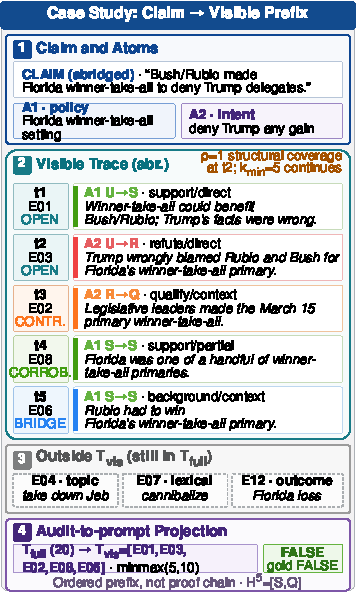
\includegraphics[width=0.98\columnwidth]{AAAI-FC-case.pdf}
\caption{An example evidence trace produced by EviTrace. Claim atoms,
selected evidence units, atom-state transitions, and the final verifier
output are shown.}
\label{fig:case}
\end{figure}


To illustrate how EviTrace organizes evidence beyond relevance
ranking, we present an example from LIAR-RAW in Figure~\ref{fig:case}.
Given the claim that ``Bush/Rubio made Florida winner-take-all because
they wanted Trump did not get anything'', the claim is decomposed into
two verifiable atoms: the existence of a winner-take-all setup and the
motivation behind the decision.

The generated trace does not simply select the most similar evidence.
Instead, each selected unit contributes to a different atom-state
transition. The first evidence unit resolves atom $A1$ through direct
support, while the second unit updates atom $A2$ from uncovered to
refuted by providing contradictory evidence. Subsequent selections add
qualifying context and complementary coverage, leading to a compact
trace containing both decisive and contextual evidence.

% 202607241248 优化表达
% In contrast, highly relevant but atom-unresolved candidates are not
% included in the final trace. This example demonstrates that the
% selector uses map-induced structural gains rather than retrieval scores
% alone, producing an ordered evidence path that exposes why each
% evidence unit is selected and how the final verification decision is
% formed.

In contrast, highly relevant but atom-unresolved candidates are not
included in the final trace. This example demonstrates that the
selector uses map-induced structural gains rather than retrieval scores
alone, producing an ordered evidence path that exposes why each unit is selected and what evidence is presented to the verifier at each stage.



\section{Conclusion}

% We introduced Map2Trace, a structure-induced framework that uses
% evidence organization itself as supervision for fact checking. It
% decomposes claims into verifiable atoms, constructs an Atom-Union
% candidate pool and a typed Evidence Map, and converts prefix-state
% transitions into pairwise preferences for a state-conditioned selector.
% Training uses neither verdict labels, gold or teacher-provided evidence
% orders, nor verifier feedback. At inference, the selector produces a
% source-linked audit trace over the full candidate pool, from which a
% separate policy forms the verifier-visible prefix.

% Under matched associated-report settings, Map2Trace outperforms
% directly comparable methods on LIAR-RAW and RAWFC and obtains the best
% tabulated development-set scores on both abstract-level SciFact metrics.
% LIAR-RAW ablations show that candidate construction, learned structural
% scoring, evidence order, and Evidence Map fields affect performance,
% while structure-conditioned stopping offers a favorable
% performance--context trade-off relative to the tested fixed-capacity
% and token-budget policies. The human audit yields a 93.5\% strict joint
% pass rate for claim atomization and characterizes Evidence Map
% annotations as useful but uncertainty-sensitive: directness is
% ordinally consistent, whereas relation labels remain
% interpretation-dependent.

% We introduce Map2Trace, a structure-induced framework that utilizes evidence organization itself as supervision for fact verification. It transforms the prefix states of atomic claims into pairwise preferences for a state-conditioned selector, enabling the selector to learn diverse utilities and select candidates that maximize structural gain/similarity gain to complete chain construction. Map2Trace does not rely on complex evidence processing methods and achieves superior performance on the metrics of LIAR-RAW, RAWFC, and the cross-domain dataset SciFact. Ablation experiments on LIAR-RAW demonstrate that candidate construction, the learned structured scoring, evidence order, and Evidence Map fields all affect performance to varying degrees; meanwhile, studies on different stopping strategies also show that dynamic evidence capacity outperforms fixed capacity under certain conditions.

We introduce \textbf{EviTrace}, an atom-state transition-guided framework
that treats evidence organization as supervision for fact checking.
EviTrace decomposes claims into verifiable atoms, constructs an Atom-Union
candidate pool and a typed atom--evidence map, and converts
prefix-dependent state transitions into pairwise preferences for a
state-conditioned selector. Without verdict labels, gold evidence
traces or verifier feedback, the selector learns to
produce an ordered trace for downstream verification.

Experiments on LIAR-RAW, RAWFC, and SciFact demonstrate the effectiveness
of EviTrace across different settings. Controlled analyses suggest that
candidate construction, transition-induced preference learning, and
evidence ordering all contribute to its performance, while
structure-conditioned stopping can provide a favorable
performance--context trade-off relative to fixed capacity. Human
evaluation further indicates that claim atomization is stable, although
Evidence Map annotations remain sensitive to uncertainty. These results
suggest that explicit evidence organization can provide useful
structural supervision for fact checking. 

% Several limitations bound these conclusions. The pipeline depends on
% LLM-generated annotations and upstream candidate recall, so atomization
% and map errors may propagate through subsequent stages; source linkage
% also does not establish source credibility. The covered-atom rate is a
% structural control signal rather than a guarantee of human or logical
% evidence sufficiency, and the audit trace records how evidence was
% organized rather than the causal basis of the verifier's prediction.
% Greedy selection is not globally optimal, the main results use single
% canonical runs, and SciFact is evaluated only on the development split.
% Future work should improve annotation calibration and source-quality
% modeling, evaluate multi-seed and held-out robustness, and develop
% stronger optimization and human-grounded criteria for evidence
% sufficiency.

% 202607241248 优化表达
% Several limitations bound these conclusions. EviTrace depends on
% LLM-generated structural annotations and upstream candidate recall; although experiments show that LLM annotations have a certain degree of consistency with human annotations, annotation bias or recall failures can still cause error propagation to subsequent stages, and the introduction of LLM annotations also incurs additional costs. Another noteworthy point is that this paper focuses solely on evidence selection and does not address how to retrieve and incorporate new additional evidence, which makes the performance on LIAR-RAW inferior to some methods that use external evidence. Meanwhile, this paper also does not address how to handle evidence conflicts; conflicting evidence serves only as a state change signal, and in terms of processing, conflicting evidence is handed over to the LLM Verifier for processing. Future work will incorporate additional evidence sources, consider low-cost approaches that do not require LLM API annotation, and construct more explicit conflict resolution strategies.

Several limitations bound these conclusions. EviTrace depends on
LLM-generated structural annotations and upstream candidate recall; although experiments show that LLM annotations have a certain degree of consistency with human annotations, annotation bias or recall failures can still cause error propagation to subsequent stages, and the introduction of LLM annotations also incurs additional costs. Another noteworthy point is that this paper focuses solely on evidence selection and does not address how to retrieve and incorporate new additional evidence, which makes the performance on LIAR-RAW inferior to some methods that use external evidence. Meanwhile, this paper also does not address how to handle evidence conflicts; conflicting evidence serves only as a state change signal, and in terms of processing, conflicting evidence is handed over to the LLM Verifier for processing. EviTrace externalizes selector-level evidence reasoning, but it should not be interpreted as a faithful record of the verifier’s latent reasoning or as a causal explanation of its prediction. Future work will incorporate additional evidence sources, consider low-cost approaches that do not require LLM API annotation, and construct more explicit conflict resolution strategies.

\bibliography{references}

\end{document}
